\begin{surferPage}{Eine Quintik mit 15 Kuspen}
   Diese Fl�che vom Grad $5$ (daher Quintik) hat $15$ $A_2$ Singularit�ten, auch Kuspen genannt; diese Quintik und eine Serie verwandter Fl�chen hat
    Oliver Labs 2005 angegeben. 
    
    Offensichtlich sehen f�nf der Singularit�ten anders aus als die
    anderen zehn.
    Die f�nf sind n�mlich $A_2^{++}$ Singularit�ten, die anderen $A_2^{+-}$:
    \vspace*{-0.3em}
    \begin{center}
      \begin{tabular}{c@{\qquad}c}
        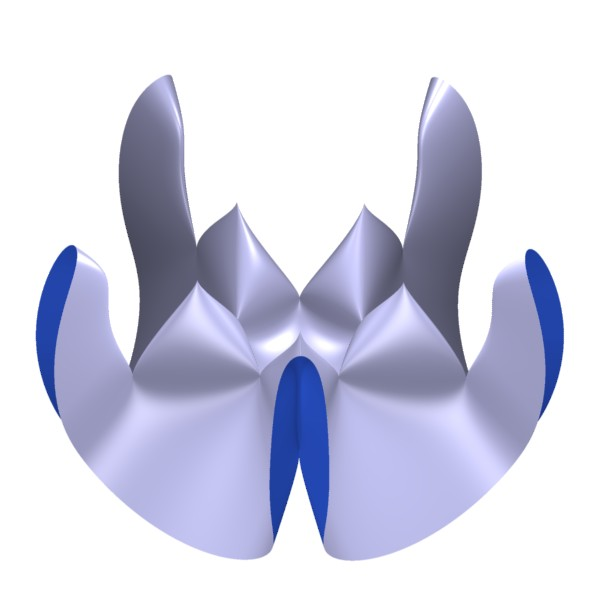
\includegraphics[height=1.2cm]{./../../common/images/dessins_quint_15a2}
        &
        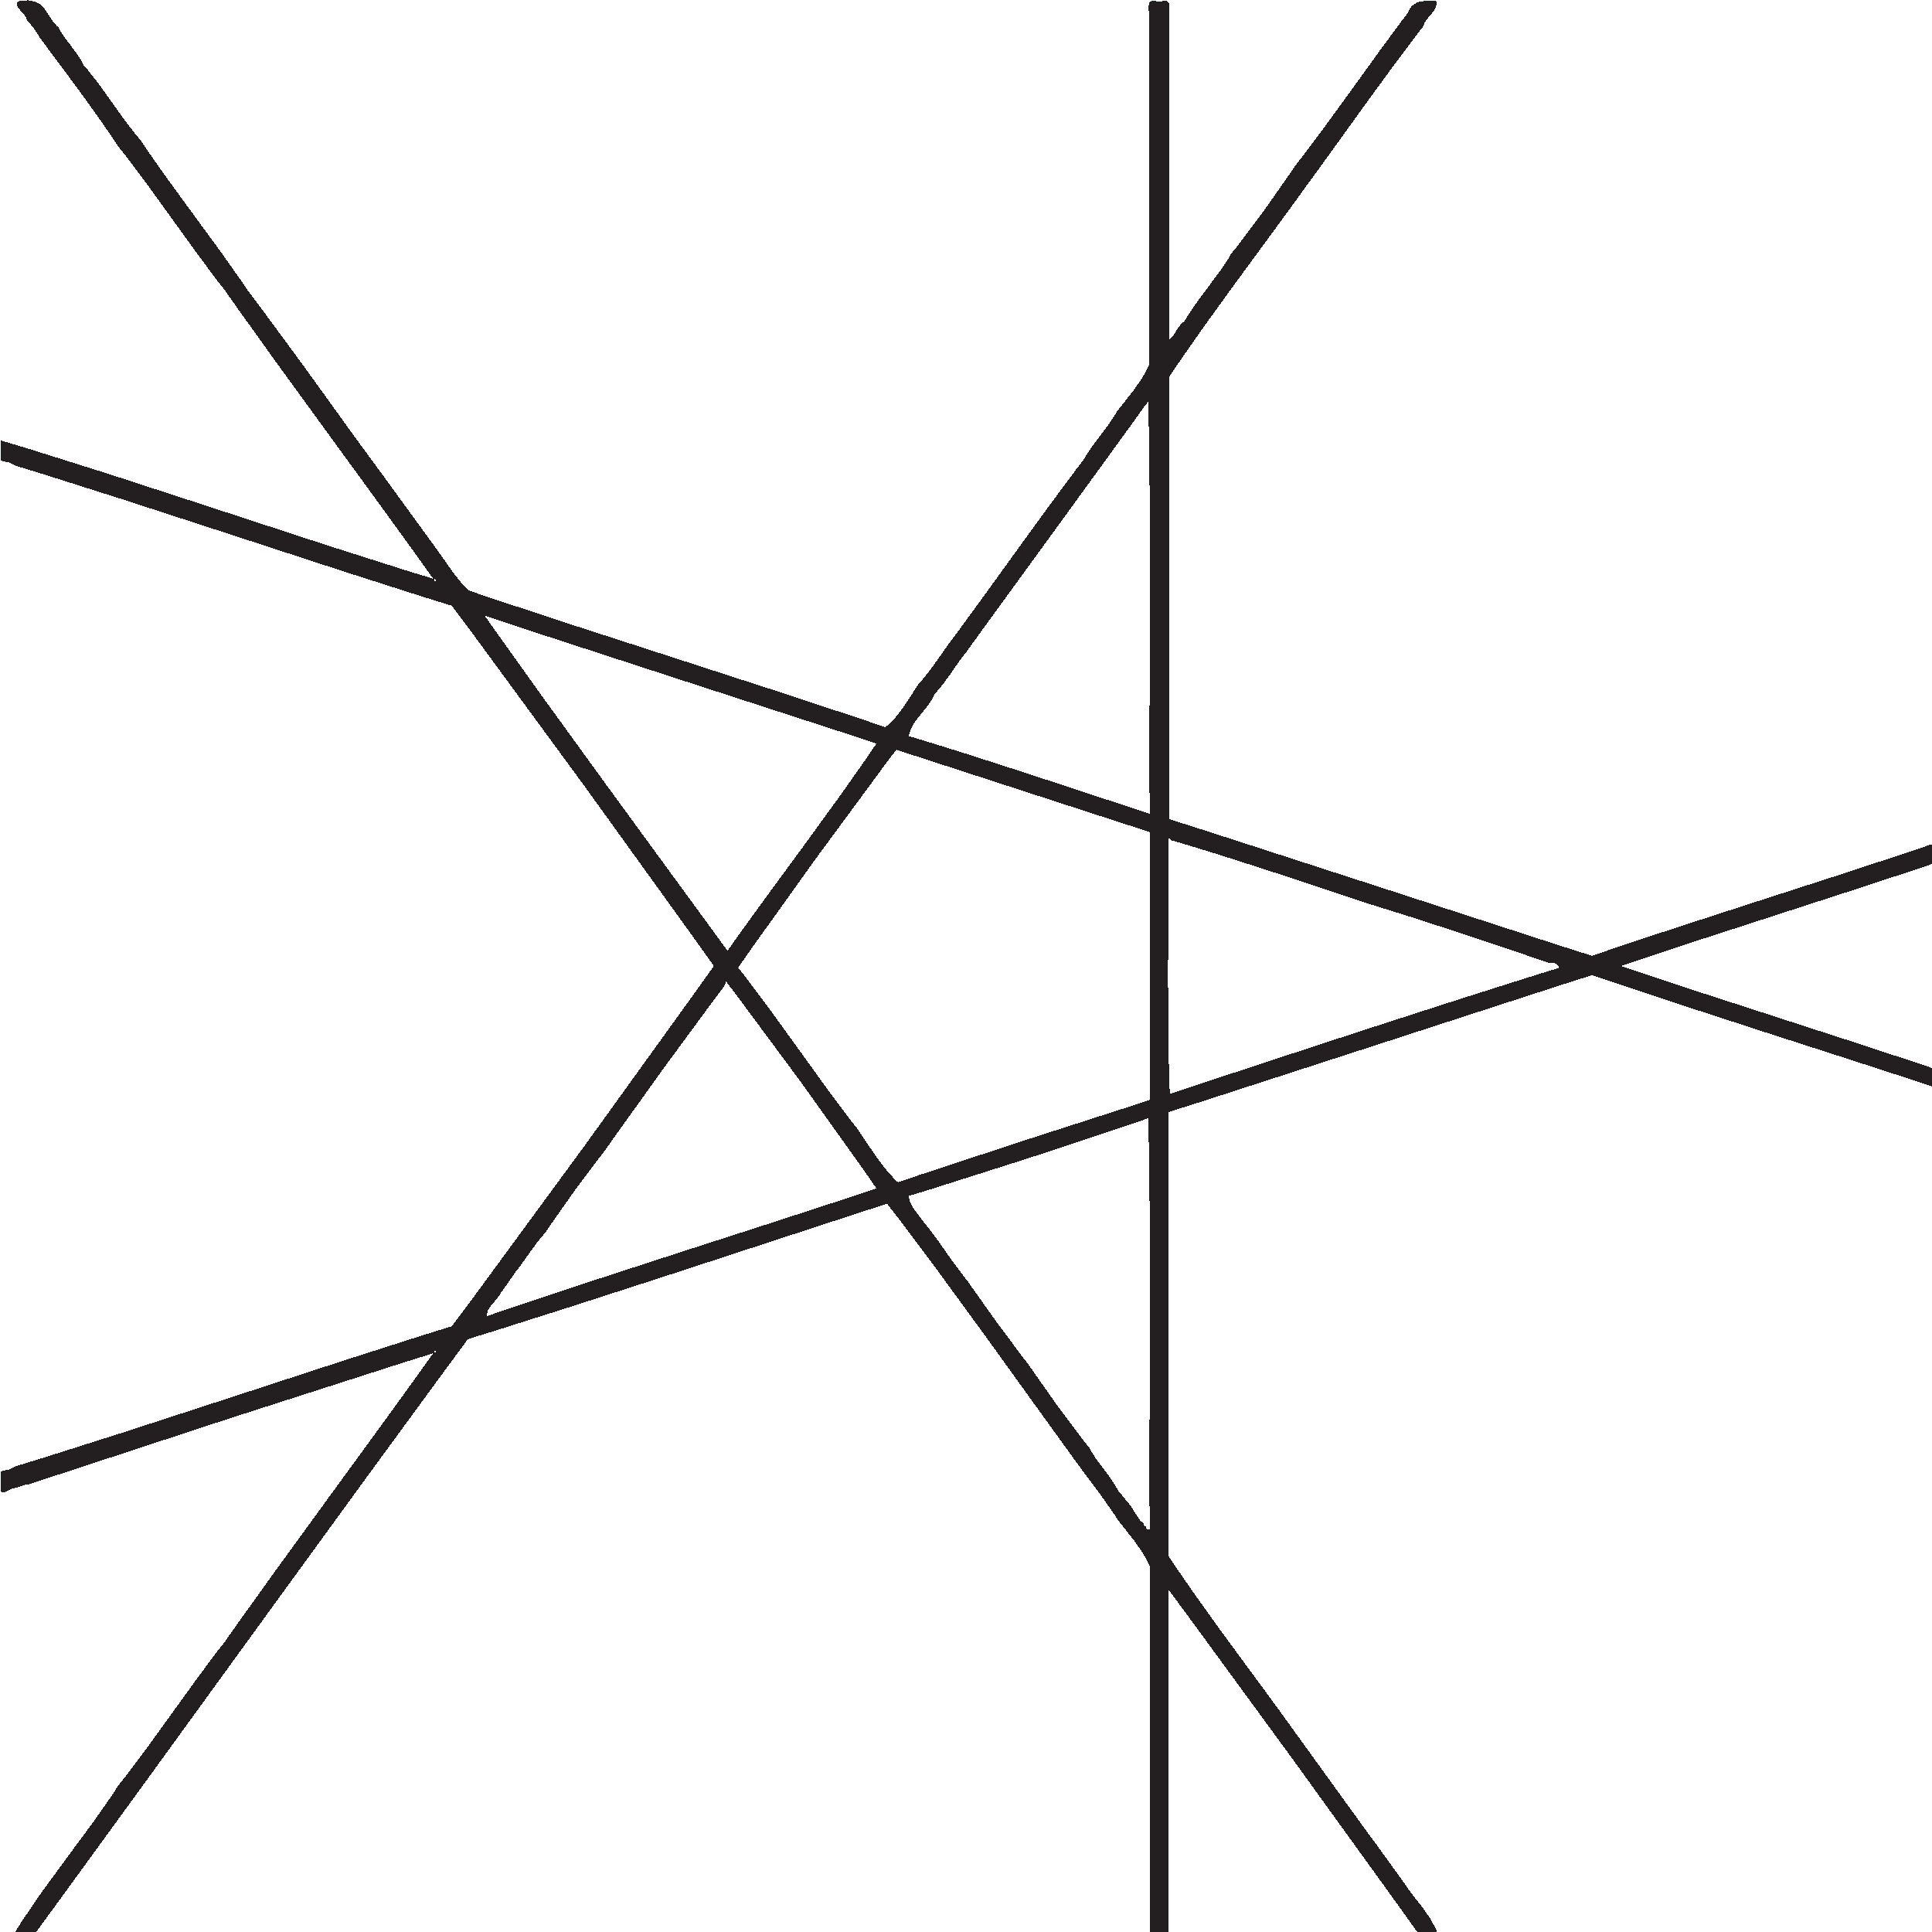
\includegraphics[height=1.2cm]{./../../common/images/rp5.pdf}
      \end{tabular}
    \end{center}
    \vspace*{-0.3em}    
    Auch diese Fl�che hat eine Gleichung der Form
    $S_5(x,y) + t(z)=0,$
    wobei $S_5(x,y)$ ein regelm��iges F�nfeck (linkes Bild) beschreibt und
    $t(z)$ eine Variante der bereits angesprochenen Tchebychev-Polynome
    ist.   

    Eine andere Quintik (links) mit $15$ Kuspen hat Wolf Barth angegeben; sie
    ist mit der Clebsch-Kubik (rechts) verwandt (beide im mittleren Bild):  
    \vspace*{-0.3em}
    \begin{center}
      \begin{tabular}{c@{\quad}c@{\quad}c}
        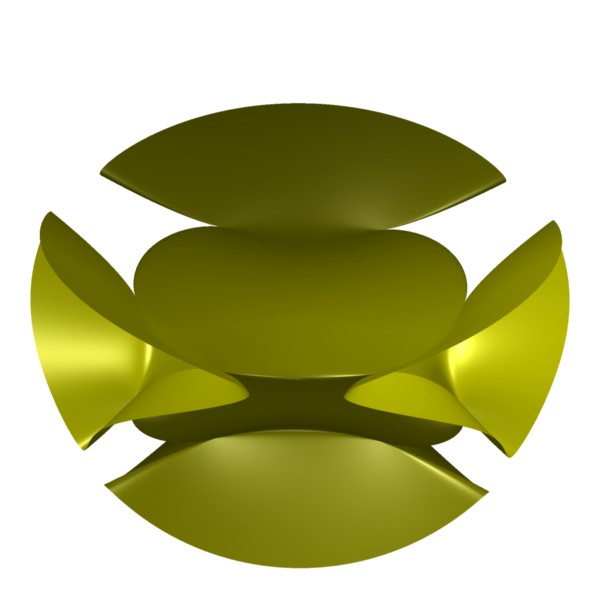
\includegraphics[height=1.2cm]{./../../common/images/barthquintic_green}
        &
        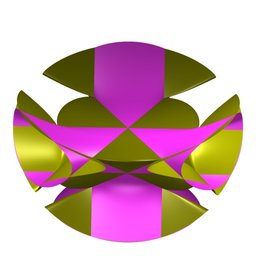
\includegraphics[height=1.2cm]{./../../common/images/barthquintic_clebschcubic}
        &
        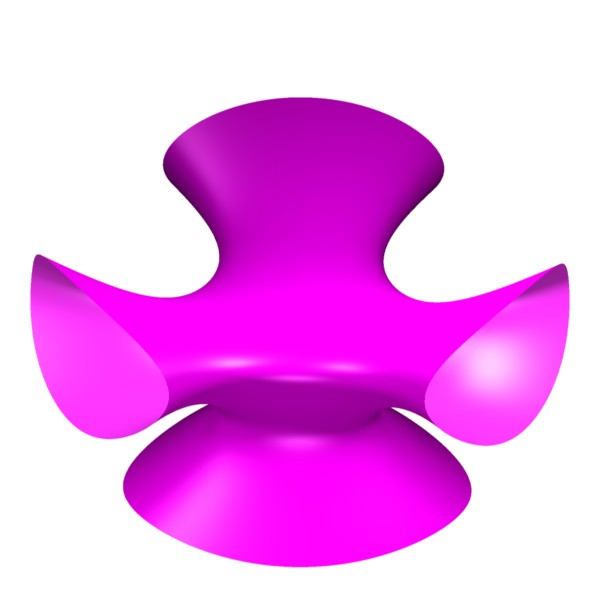
\includegraphics[height=1.2cm]{./../../common/images/clebschcubic_pink}
      \end{tabular}
    \end{center}
    \vspace*{-0.3em}
\end{surferPage}